\documentclass[utf8,russian]{beamer}
\usepackage[T2A]{fontenc}
\usepackage[utf8]{inputenc}
\usepackage[russian]{babel}
\usepackage{graphicx}
\usepackage{booktabs}

% Настройка темы Beamer
\usetheme{Madrid}
\usecolortheme{whale}
\setbeamertemplate{navigation symbols}{} % Убираем навигационные символы

% Информация о презентации
\title[Доклад по ЕСПД]{Стандарты ЕСПД: ГОСТ 19.502-78 и ГОСТ 19.005-85}
\subtitle{Анализ актуальности и основных требований}
\author[Егоров А.В.]{Выполнил: Егоров А.В.\\Группа: М3О-225БВ-24\\Кафедра 304}
\institute[МАИ]{Московский авиационный институт\\(национальный исследовательский университет)}
\date[02.07.2026]{2 июля 2026 г.}

\begin{document}

% 1. Титульный слайд
\begin{frame}
  \titlepage
\end{frame}

% 2. Слайд "Цели и задачи"
\begin{frame}{Введение}
  \begin{block}{Цели работы}
    \begin{itemize}
      \item Анализ актуальности стандартов ГОСТ 19.502-78 и ГОСТ 19.005-85 по фондам нормативных документов библиотеки МАИ.
      \item Изучение требований Единой системы программной документации (ЕСПД) к содержанию документа «Описание программы» и правилам построения схем алгоритмов.
    \end{itemize}
  \end{block}
  
  \begin{block}{Практическое значение}
    Соблюдение данных стандартов является обязательным условием при оформлении комплекта программной документации к разрабатываемому программному продукту по курсу технологической практики.
  \end{block}
\end{frame}

% 3. Слайд "Проверка актуальности стандартов"
\begin{frame}{Проверка актуальности стандартов в библиотеке МАИ}
  По результатам проверки действующего четырёхтомника стандартов в кабинете нормативных документов библиотеки МАИ (корпус 7):
  \begin{itemize}
    \item \textbf{ГОСТ 19.502-78} — \textbf{Действует} (внесено Изменение №1 от 1-XI-1981).
    \item \textbf{ГОСТ 19.005-85} — \textbf{Действует} (без изменений).
  \end{itemize}
  \vfill
  \textit{Примечание:} Для сравнения, соседний стандарт ГОСТ 19.101-77 заменён на ГОСТ 19.101-2024 с 30.01.2025 г., однако рассматриваемые стандарты сохраняют полную силу.
\end{frame}

% 4. Слайд "Фото подтверждение 1"
\begin{frame}{Фото подтверждение: ГОСТ 19.502-78}
  \begin{figure}[h]
    \centering
    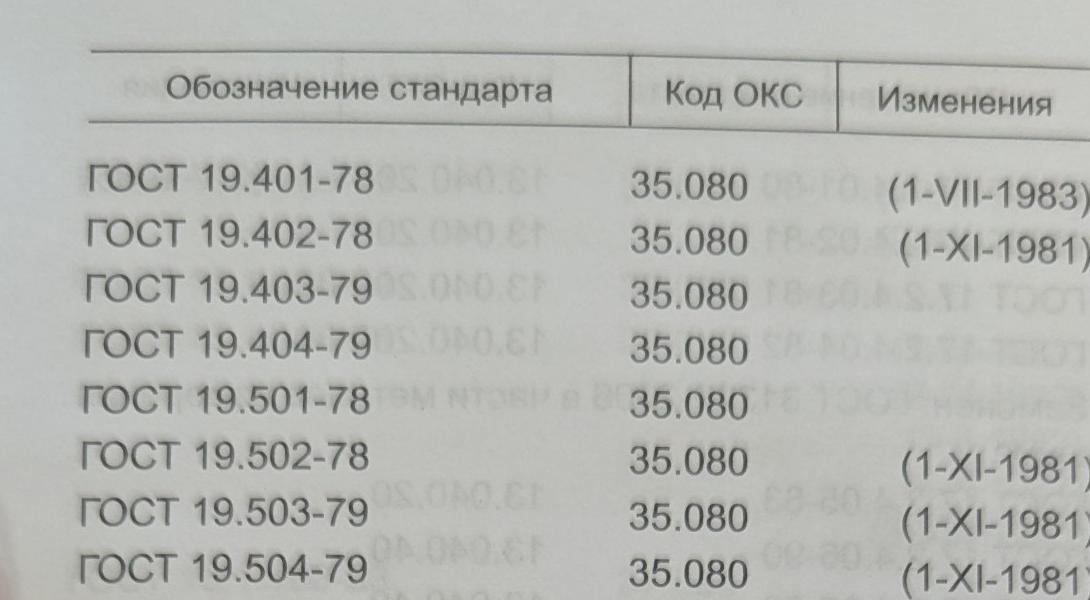
\includegraphics[width=0.85\textwidth]{gost-19.502-78-crop.jpg}
    \caption{Строка стандарта ГОСТ 19.502-78 из каталога библиотеки}
  \end{figure}
\end{frame}

% 5. Слайд "Фото подтверждение 2"
\begin{frame}{Фото подтверждение: ГОСТ 19.005-85}
  \begin{figure}[h]
    \centering
    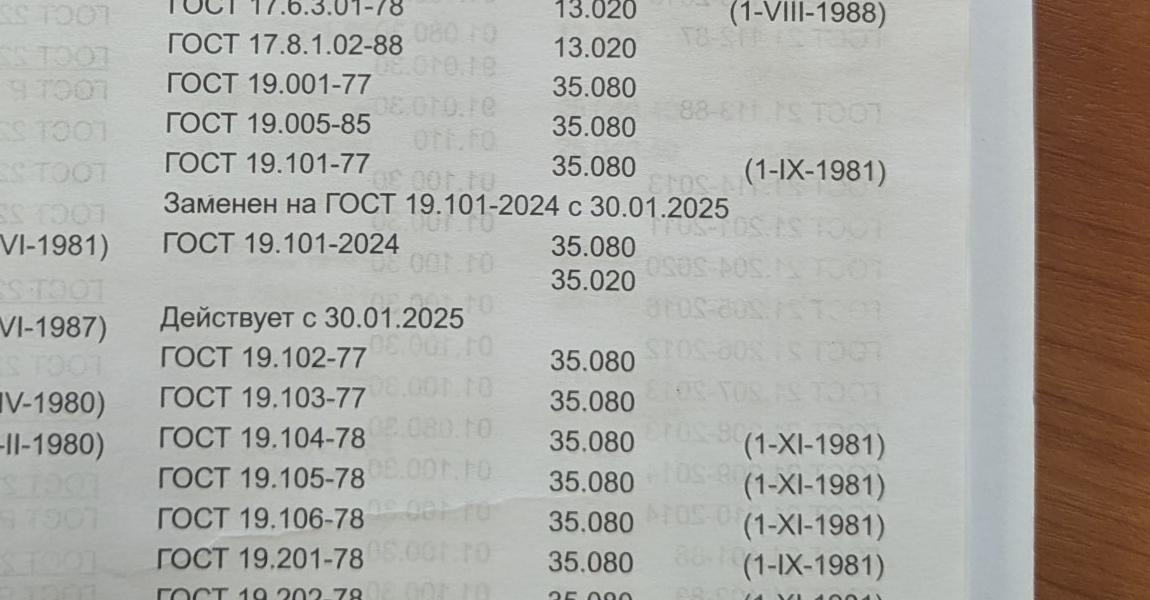
\includegraphics[width=0.85\textwidth]{gost-19.005-85-crop.jpg}
    \caption{Строка стандарта ГОСТ 19.005-85 из каталога библиотеки}
  \end{figure}
\end{frame}

% 6. Слайд "ГОСТ 19.502-78 Описание программы"
\begin{frame}{ГОСТ 19.502-78: Описание программы}
  Стандарт определяет требования к содержанию и оформлению программного документа \textbf{«Описание программы»}.
  \vfill
  \begin{block}{Обязательная структура документа}
    \begin{enumerate}
      \item \textbf{Общие сведения}: обозначение, наименование программы, требования к программному и аппаратному окружению.
      \item \textbf{Функциональное назначение}: классы решаемых задач, ограничения на применение.
      \item \textbf{Описание логики}: схемы алгоритмов, структура программы, описание модулей и связей между ними.
      \item \textbf{Вызываемые программы и системные средства}.
      \item \textbf{Характеристики программы}: объёмы памяти, быстродействие.
      \item \textbf{Набор данных}: входные и выходные форматы.
      \item \textbf{Настройка и проверка}: тесты и проверка работоспособности.
    \end{enumerate}
  \end{block}
\end{frame}

% 7. Слайд "ГОСТ 19.005-85 Схемы алгоритмов"
\begin{frame}{ГОСТ 19.005-85: Схемы алгоритмов и программ}
  Стандарт определяет условные обозначения и правила выполнения схем алгоритмов, программ и данных (родственный стандарт — ГОСТ 19.701-90 / ИСО 5807-85).
  \vfill
  \begin{block}{Основные графические символы процессов}
    \begin{itemize}
      \item \textbf{Процесс} (прямоугольник) — выполнение операции или группы операций, изменяющих данные.
      \item \textbf{Решение} (ромб) — определение направления выполнения алгоритма в зависимости от условий (ветвление).
      \item \textbf{Предопределенный процесс} (прямоугольник с двойными боковыми границами) — вызов вспомогательного алгоритма (функции).
      \item \textbf{Терминатор} (скругленный прямоугольник) — пуск, останов, вход или выход из программы.
      \item \textbf{Ввод-вывод} (параллелограмм) — преобразование данных в форму, пригодную для обработки.
    \end{itemize}
  \end{block}
\end{frame}

% 8. Слайд "Правила построения схем"
\begin{frame}{ГОСТ 19.005-85: Правила выполнения схем}
  \begin{itemize}
    \item \textbf{Линии потоков}: направляются сверху вниз и слева направо. Если направление отличается, на линиях обязательно ставятся стрелки.
    \item \textbf{Надписи в блоках}: формулируются кратко на естественном языке, математическими формулами или псевдокодом.
    \item \textbf{Нумерация блоков}: выполняется в левом верхнем углу символа для ссылок в текстовом описании программы.
    \item \textbf{Пересечение линий}: допускается, но не должно ухудшать читаемость схемы. Желательно использовать соединители (круглые элементы перехода).
  \end{itemize}
  \vfill
  \begin{center}
    \textit{Схемы алгоритмов служат основой для документирования структуры программы и её логики в рамках ГОСТ 19.402-78 и ГОСТ 19.502-78.}
  \end{center}
\end{frame}

% 9. Слайд "Заключение"
\begin{frame}{Заключение}
  \begin{block}{Выводы}
    \begin{itemize}
      \item Проведённый библиотечный аудит показал актуальность стандартов ГОСТ 19.502-78 и ГОСТ 19.005-85 на 2026 год.
      \item Совместное использование этих стандартов позволяет создать качественный программный документ «Описание программы», содержащий наглядные и стандартизированные схемы работы алгоритмов.
      \item Разработанная по варианту 5 C++ программа полностью соответствует правилам структурного программирования и сопровождается комплектом документации ЕСПД в формате LaTeX.
    \end{itemize}
  \end{block}
  \vfill
  \begin{center}
    \Large Спасибо за внимание!\\
    \large Вопросы?
  \end{center}
\end{frame}

\end{document}
